
\section{Conjuntos}

En la sección anterior, hemos definido la noción de predicado como una expresión que depende de variables que al ser reemplazadas por \textbf{elementos} de un \textbf{conjunto} de referencia lo transforman en una proposición lógica. Sin embargo, no hemos definido formalmente la noción de \textit{conjunto}. 

En este curso, no veremos teoría axiomática de conjuntos, si no que entenderemos un conjunto como una \textit{colección de cosas}, sus elementos. Más bien, estudiaremos como obtener nuevos conjuntos a partir de otros dados o conocidos. 

\subsection{Definiciones preliminares}

\begin{definicion}
	\textbf{(Universo)}
	Asumiremos la existencia de un conjunto de referencia que usualmente denotaremos $E$ y al que pertenecen todos los elementos con los que se va a trabajar. A este conjunto lo llamamos \textbf{universo} y asumiremos que siempre contiene al menos un elemento. 
	
	Formalmente, $E$ es tal que la función proposicional $e\in E$ es siempre verdadera. Muchas veces, $E = \N$ o $E = \R$. 
\end{definicion}

\begin{definicion}
	\textbf{(Vacío)}
	Existe un conjunto, el \textbf{conjunto vacío} (denotado por $\phi$) que no contiene elementos. Es decir, $\forall x \in E, x \in \phi \iff F$. 
\end{definicion}

\begin{definicion}
	\textbf{(Igualdad)}
	Diremos que los conjuntos $A$ y $B$ son \textbf{iguales}, denotado $A=B$, si $A$ y $B$ tienen exactamente los mismos elementos. Es decir: 
	$$ A = B \iff \forall x \in E, (x \in A \iff x \in B ) $$ 
\end{definicion}

\begin{definicion}
	\textbf{(Inclusión)}
	Se dice que $A$ es subconjunto de $B$ (o que $A$ está contenido en $B$), denotado $A\subseteq B$, si todos los elementos de $A$ están también en $B$. Es decir: 
	$$ A \subseteq B \iff \forall x \in E, (x \in A \Longrightarrow x \in B) $$ 
\end{definicion}

\begin{figure}[H]
	\begin{center}
		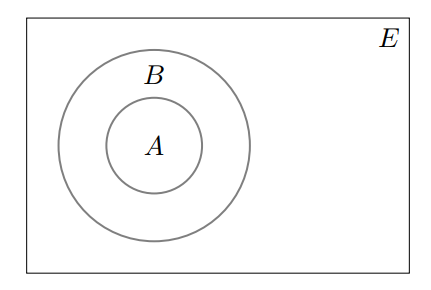
\includegraphics[scale=0.8]{figuras/capitulo1/02-conjuntos/inclusion.png}
		\caption{$A \subseteq B$}
		%\label{fig:1_2_inclusion}
	\end{center}
\end{figure}

\begin{proposicion}
		\textbf{(Propiedades de la igualdad)}
		Para $A, B, C \subseteq E$ se cumplen las siguientes propiedades: 
		\begin{itemize}
			\item Reflexividad: $A = A$. 
			\item Simetría: $A = B \iff B  = A$. 
			\item Transitividad: $A = B \y B = C \Longrightarrow A = C$. 
		\end{itemize}
\end{proposicion}

\begin{proposicion}
	\textbf{(Propiedades de la inclusión)}
	Para $A, B, C \subseteq E$ se cumplen las siguientes propiedades: 
	\begin{itemize}
		\item Reflexividad: $A \subseteq A$. 
		\item Antisimetría: $A = B \iff A \subseteq B \y B \subseteq A$. 
		\item Transitividad: $A \subseteq B \y B \subseteq C \Longrightarrow A \subseteq C$. 
	\end{itemize}
\end{proposicion}

\begin{proposicion}
	Para cualquier conjunto $A$ se tiene que: 
	$$ \phi \subseteq A \subseteq E $$ 
\end{proposicion}

\subsection{Álgebra de conjuntos}

\begin{definicion}
	\textbf{(Unión)}
	Sean $A$ y $B$ conjuntos. La \textbf{unión} de $A$ y $B$, denotada $A\cup B$, es el conjunto que reúne a todos los elementos que están en $A$ y a todos los elementos que están en $B$. Formalmente, 
	$$ \forall x \in E, x \in A \cup B \iff x \in A \o x \in B $$ 
\end{definicion}


\begin{figure}[H]
	\begin{center}
		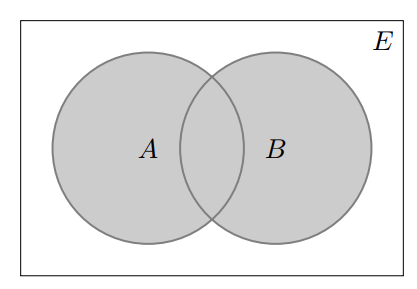
\includegraphics[scale=0.8]{figuras/capitulo1/02-conjuntos/union.png}
		\caption{$A \cup B$}
		%\label{fig:1_2_inclusion}
	\end{center}
\end{figure}

\begin{definicion}
	\textbf{(Intersección)}
	Sean $A$ y $B$ conjuntos. La \textbf{intersección} de $A$ y $B$, denotada $A\cap B$, es el conjunto de los elementos que están tanto en $A$ como en $B$. 
	$$ \forall x \in E, x \in A \cap B \iff x \in A \y x \in B $$ 
\end{definicion}

\begin{figure}[H]
	\begin{center}
		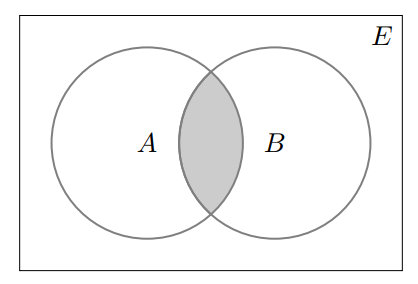
\includegraphics[scale=0.8]{figuras/capitulo1/02-conjuntos/interseccion.png}
		\caption{$A \cap  B$}
		%\label{fig:1_2_inclusion}
	\end{center}
\end{figure}

\begin{proposicion}
	Sean $A, B, C$ conjuntos. Se tiene que: 
	\begin{itemize}
		\item $A \cap B \subseteq A \subseteq A \cup B$. 
		\item $A \subseteq B \y A \subseteq C \Longrightarrow A \subseteq B \cap C$. 
		\item $A \subseteq B \y C \subseteq B \Longrightarrow A \cup C \subseteq B$. 
	\end{itemize}
\end{proposicion}

\begin{proof}
	Mostraremos cada proposición por separado: 
	\begin{itemize}
		\item Veamos que: $$ A \cap B \subseteq A \subseteq A \cup B$$ 
		En efecto, si $x \in A \cap B$, por definición:
		$$ x \in A \y x \in B $$ 
		Si $x\in A$, entonces la proposición 
		$$ x \in A \o x \in B$$
		Es verdadera. Como esto último equivale a $A \subseteq A \cup B$ se obtiene la propiedad.
		
		\item Veamos ahora que: 
		$$A \subseteq B \y A \subseteq C \Longrightarrow A \subseteq B \cap C$$
		Sea $x \in A$. Debemos mostrar que $x \in B\cap C$. 
		
		En efecto, como $x \in A$ y $A \subseteq B$, entonces $x \in B$. De manera análoga $x \in C$. Es decir: 
		$$ x \in B \y x\in C$$ 
		Equivalentemente: 
		$$ x \in B \cap C $$
		Se concluye entonces que: 
		$$ A \subseteq B \cap C $$ 
		
		\item \textcolor{red}{La tercera parte de la demostración queda propuesta.}
	\end{itemize}
\end{proof}


\begin{proposicion}
	Sean $A, B$ dos conjuntos tales que $A \subseteq B$. Entonces: 
	$$ A \cup B = B \quad \y \quad A \cap B = A $$ 
\end{proposicion}

\begin{proof}
	Veremos que $A \subseteq B$ implica que $ A \cup B = B$. 
	En efecto:
	$$ A \subseteq B \iff A \subseteq B \y B \subseteq B $$ 
	$$ \Longrightarrow \quad A \cup B \subseteq B $$ 
	$$ \Longrightarrow \quad A \cup B = B $$ 
	El resto de la demostración se construye de manera similar. 
\end{proof}

\begin{proposicion}
	Sean $A, B, C$ conjuntos. Se tienen las siguientes igualdades: 
	\begin{itemize}
		\item $A \cup A  = A, \quad A\cup A = A$. 
		\item $A \cup \phi = A$. 
		\item $A \cap \phi = \phi$. 
		\item $A \cap E = A$. 
		\item $A \cup E = E$. 
		\item $A \cup B = B \cup A$. 
		\item $A \cap B = B \cap A$. 
		\item $A \cup (B \cap C) = ( A \cup B ) \cup C$. 
		\item $A \cap (B \cap C) = (A \cap B) \cap C$. 
		\item $A \cup (B \cap C) = (A\cup B) \cap (A\cup C)$. 
		\item $A \cap (B \cup C) = (A \cap B) \cup (A \cap C)$.  
	\end{itemize}
\end{proposicion}


\begin{proof}
	\textcolor{red}{to be added..}
\end{proof}

\begin{definicion}{(Conjunto complemento)}
	El complemento de un conjunto $A$ (con respecto a $E$), denotado $A^c$ es el conjunto de todos los elementos que están en $E$, pero no están en $A$. Formalmente: 
	$$ \forall x \in E, x \in A^c \quad \iff \quad x \notin A $$ 
\end{definicion}

\begin{figure}[H]
	\begin{center}
		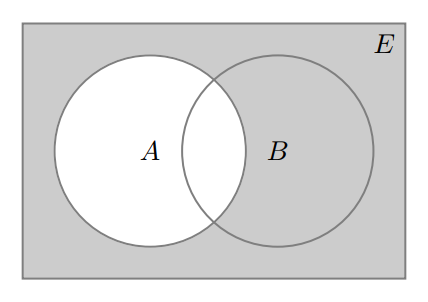
\includegraphics[scale=0.8]{figuras/capitulo1/02-conjuntos/complemento.png}
		\caption{$A^c$}
		%\label{fig:1_2_inclusion}
	\end{center}
\end{figure}

\begin{proposicion}
	Se tiene que: 
	\begin{itemize}
		\item $(A \cup B)^c = A^c \cap B ^c$ 
		\item $(A \cap B)^c = A^c \cup B^c$. 
		\item $A \cap A^c = \phi$ 
		\item $A \cup A^c = E$. 
	\end{itemize}

\end{proposicion}
\begin{definicion}
	\textbf{(Diferencia)}
	La diferencia de $A$ con $B$, que notamos $A \setminus B$, es el conjunto formado por elementos que están en $A$ y que no están en $B$. Formalmente: 
	$$ A\setminus B = A \cap B ^c $$ 
\end{definicion}

\begin{figure}[H]
	\begin{center}
		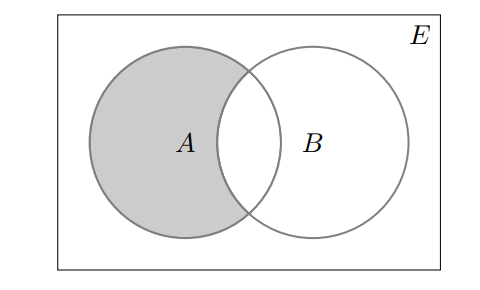
\includegraphics[scale=0.8]{figuras/capitulo1/02-conjuntos/diferencia.png}
		\caption{$A\setminus B$}
		%\label{fig:1_2_inclusion}
	\end{center}
\end{figure}

\begin{definicion}
	\textbf{(Unión sobre conjuntos de índices)}
	Sea $\Lambda$ un conjunto de índices y, $\forall \lambda \in \Lambda$, sea $A_\lambda \subseteq E$ un conjunto. Se define la unión de los $A_\lambda$ con $\lambda \in \Lambda$, denotado $\bigcup_{\lambda \in \Lambda} A_\lambda$, como el conjunto de los $x$ tal que $x \in A_\lambda$ para algún $\lambda \in \Lambda$. Formalmente: 
	$$ \forall x \in E , x\in \bigcup_{\lambda \in \Lambda} A_\lambda \quad \iff \quad \exists \lambda \in \Lambda , x \in A_\lambda$$ 
\end{definicion}	

\begin{definicion}
	\textbf{(Intersección sobre conjuntos de índices)}
	Sea $\Lambda$ un conjunto de índices y, $\forall \lambda en \Lambda$, sea $A_\lambda \subseteq E$ un conjunto. Se define la intersección de los $A_\lambda$ con $\lambda \in \Lambda$, denotado $\bigcap_{\lambda \in \Lambda} A_\lambda$, como el conjunto de los $x$ tal que $x \in A_\lambda$ para todo $\lambda \in \Lambda$. Formalmente: 
	$$ \forall x \in E , x\in \bigcap_{\lambda \in \Lambda} A_\lambda \quad \iff \quad \exists \lambda \in \Lambda , x \in A_\lambda$$ 
\end{definicion}

\subsection{Referencias}

\textcolor{red}{Apunte Introducción al Álgebra, semana 3. }	